% tikzpic.tex
\documentclass[crop,tikz]{standalone}% 'crop' is the default for v1.0, before it was 'preview'
%\usetikzlibrary{...}% tikz package already loaded by 'tikz' option
\usepackage{amsmath,amsthm,amssymb,mathrsfs,amsfonts,dsfont}

\begin{document}
    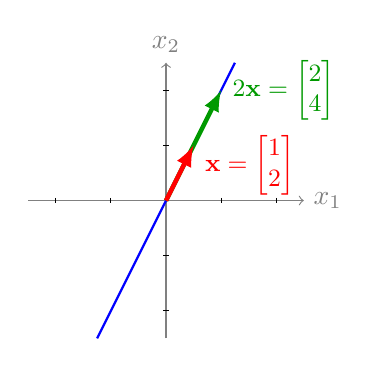
\begin{tikzpicture}[scale=0.35]
        \draw[->, gray] (-5,0) -- (5,0) node[right] {$x_1$};
        \draw[->, gray] (0,-5) -- (0,5) node[above] {$x_2$};
        \foreach \x in {-4,-2,2,4}
        \draw (\x,0.1) -- (\x,-0.1);
        \foreach \y in {-4,-2,2,4}
        \draw (0.1,\y) -- (-0.1,\y);
        % Plot an example point and its corresponding arrow
        \draw[thick, blue] (-2.5,-5) --  (2.5,5);
        
        \draw[-latex, ultra thick, black!40!green] (0,0) --  (2,4) node[font=\small, right, yshift=-0.0cm, black!40!green] {$2\mathbf{x} = \begin{bmatrix} 2 \\ 4 \end{bmatrix}$}; % Arrow with label

        \draw[-latex, ultra thick, red] (0,0) --  (1,2) node[font=\small, right, yshift=-0.25cm, red] {$\mathbf{x} = \begin{bmatrix} 1 \\ 2 \end{bmatrix}$}; % Arrow with label
    \end{tikzpicture}
\end{document}